\documentclass[conference]{IEEEtran}

\usepackage{graphicx}
\usepackage[caption=false]{subfig}

\def\shell{\tt}

\title{{\bf DAT110: The Methods Course}\\
       \vspace{0.2cm}
       Quick Start Guide for \LaTeX\\
       \vspace{0.4cm}
       \normalsize Version 20221006}
\author{\normalsize Per Larsson-Edefors \\
        \normalsize Chalmers University of Technology
        }

%------------------

\begin{document}

\maketitle

\section{Introduction}

\LaTeX, or simply LaTeX in the following, is an often used system
for creating scientific documents such as papers and reports. In
LaTeX, it is efficient to work with at least two different source
files, one for the text ({\shell .tex}) and one for the bibliography
({\shell .bib}).


\section{Compiling LaTeX Files}
\label{sec:compiling}

We have the option to use figure files based on the ({\shell .eps})
or the ({\shell .pdf}) formats. The Encapsulated PostScript format
used to be very common, but nowadays Adobe's Portable Document
Format is overtaking EPS (read more about figures in
Sec.~\ref{sec:figures}). As a default thus, to compile a LaTeX
document that is based on PDF figures, we use the pdflatex software
in the Linux environment. The following flow assumes we have one
file {\shell latex\_guide.tex} that refers to a bibliography file.

\begin{verbatim}
  pdflatex latex_guide
  bibtex latex_guide
  pdflatex latex_guide
  pdflatex latex_guide
\end{verbatim}

The bibliography is further described in Sec.~\ref{sec:bib}.

\section{Structure of .tex Files}

Start by defining the document class, i.e., {\it conference} as far
as reports in DAT110 are concerned. Then define any packages and
style files that you wish to utilize. Individual parameters set in
the previous step may be fine tuned, e.g., by adding

\begin{verbatim}
  \setlength{\parskip}{.8ex}
  \setlength{\parindent}{0ex}
\end{verbatim}

we reset the parindent parameter, to avoid indentation of new
paragraphs which otherwise is default for many document classes, and
instead use a leading space.

Next we state title and authors followed by the document body
which is defined to start and end using

\begin{verbatim}
  \begin{document}
  ...
  \end{document}
\end{verbatim}


\subsection{Abstract}

Prior to the introduction we can add an abstract to summarize
a report.

\begin{verbatim}
  \begin{abstract}
  ...
  \end{abstract}
\end{verbatim}


\subsection{Sections}

In a report we typically find sections such as Introduction,
Background, Method, a section describing the contributions,
Evaluation and Results, Conclusion, and Bibliography.  You can
create an introductory section by using

\begin{verbatim}
  \section{Introduction}
  ...
\end{verbatim}

You can create a subsection within the section by using

\begin{verbatim}
  \subsection{An In-Depth Study}
  ...
\end{verbatim}

If you do not want to number a headings that you create, you can
suppress numbering by adding a star

\begin{verbatim}
  \subsection*{An In-Depth Study}
  ...
\end{verbatim}


\subsection{Tables}

It takes some effort to create tables in LaTeX but in exchange the
final result can be excellent, as shown in
Table~\ref{tab:some_data}.

\begin{table}[h!]
\centering
  \def\arraystretch{1.05}
  \addtolength{\tabcolsep}{-2pt}
  \small{
  \caption{Normalized Area and Energy Overheads}
  \begin{tabular}{|l|c|c|c|}                                                   \hline
      \bf SRAM Block       & \bf Area & \bf Read Energy & \bf Total Line    \\
      \bf [rows x columns] &          & \bf per Access  & \bf Fetch Energy  \\ \hline \hline
      128 x 256b           &  1.91    & 4.15            & 1.43              \\ \hline
      256 x 128b           &  1.30    & 2.87            & 1.26              \\ \hline
      1024 x 32b           &  1.00    & 1.00            & 1.00              \\ \hline
  \end{tabular}
  \label{tab:some_data}
  }
\end{table}


\subsection{Figures}
\label{sec:figures}

Remember to store all figures that you develop in a lossless format.
As an example, Fig.~\ref{fig:vectorized_picture} shows a figure that
is stored in a vectorized format, while
Fig.~\ref{fig:compressed_picture} shows what happens if you work
with JPG files.

\begin{figure}[h!]
  \centering
  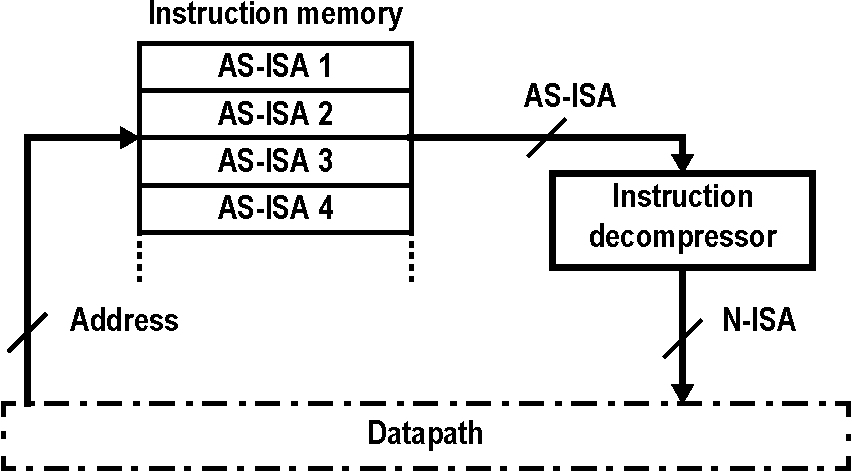
\includegraphics[width=0.8\columnwidth]{figures/figure}
  \caption{This picture was initially stored in a lossless format.}
  \label{fig:vectorized_picture}
\end{figure}


\begin{figure}[h!]
  \centering
  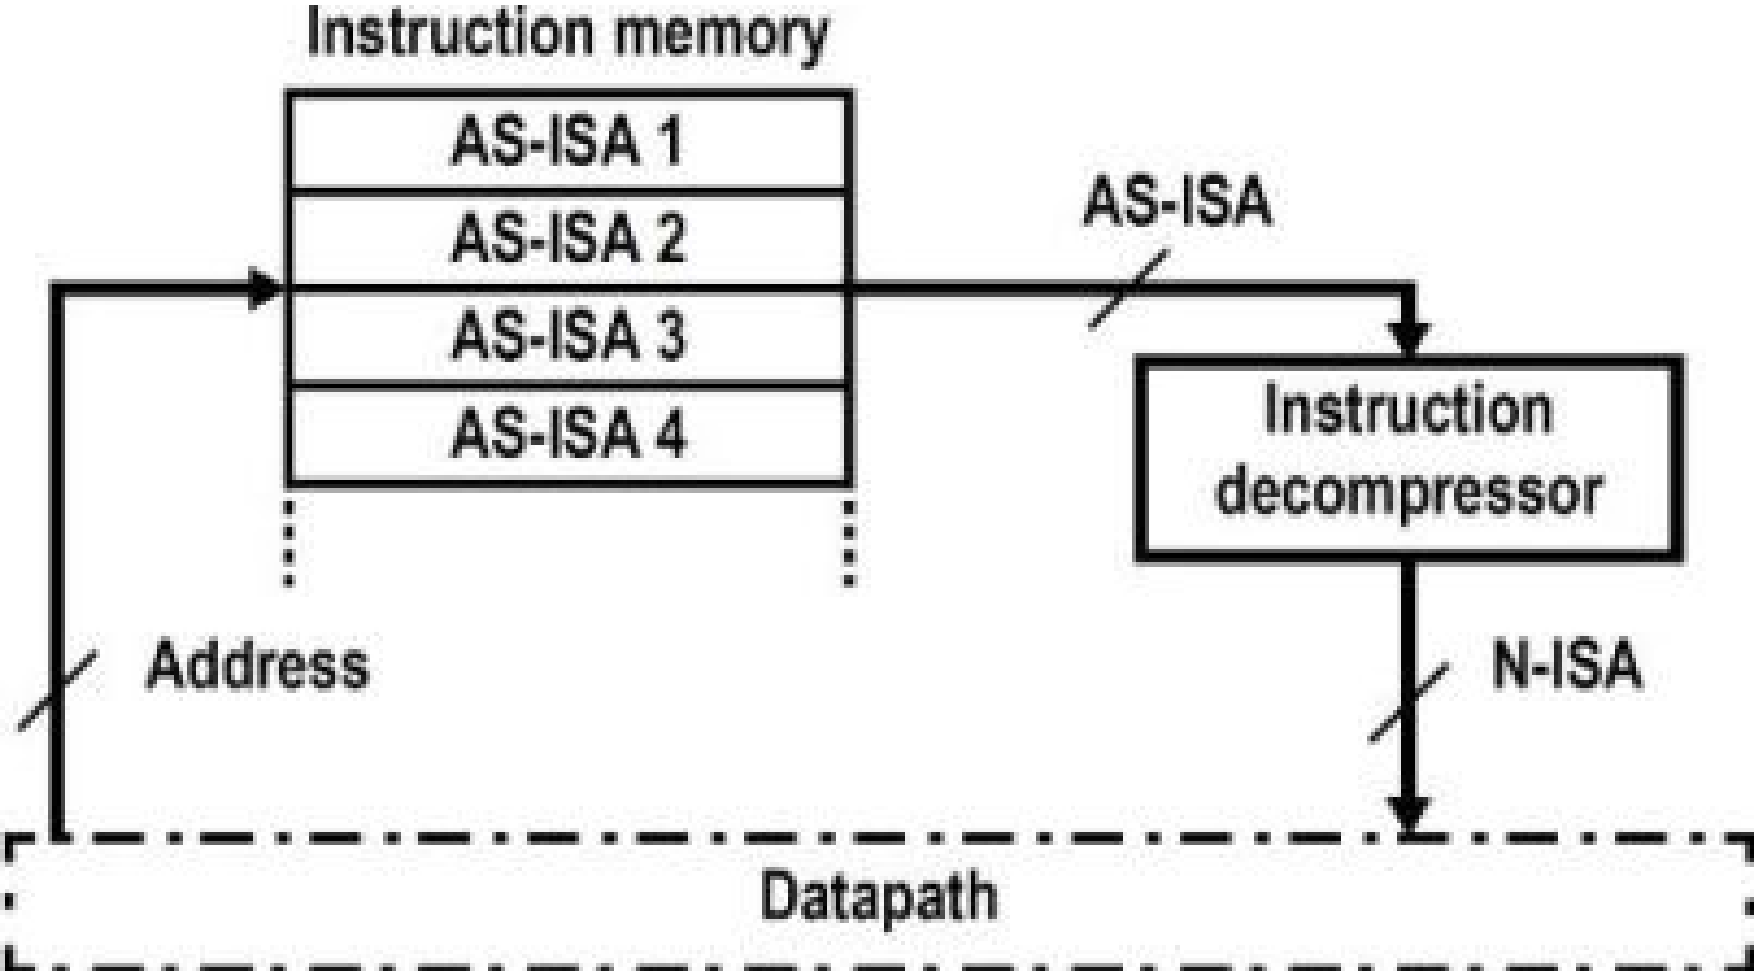
\includegraphics[width=0.8\columnwidth]{figures/figure_compressed}
  \caption{In an intermediate step, this picture was stored in a lossy JPG format.}
  \label{fig:compressed_picture}
\end{figure}

As far as software, Linux offers a few environments that support
editing block diagram figures. An older alternative is {\shell
xfig}, while a newer one is {\shell inkscape}.


\section{Using a Bibliography}
\label{sec:bib}

You collect all reference information under different BibTeX
items in a {\shell .bib} file. The reference list, as it
appears in the report, will be organized and formatted in a way
that depends on the chosen bibliography style. Since the IEEE
bibliography style is a common style in our technical area, we
use this. The two lines below are given at the end of this
file, invoking first the bibliography style and then calling
the {\shell .bib} file:

\begin{verbatim}
  \bibliographystyle{IEEEtran}
  \bibliography{refs}
\end{verbatim}

For textbook references, you add a book-type item in the {\shell
.bib} file by giving the following essential entries of information:

\begin{verbatim}
@book{*,
  AUTHOR =    {*},
  TITLE =     {*},
  PUBLISHER = {*}
  YEAR =      {*},
}
\end{verbatim}


When you refer to a chapter in book which contains several
chapters written by different authors and which has been
compiled by editors, you use the incollection entry:

\begin{verbatim}
@incollection{*,
  AUTHOR =    {*},
  TITLE =     {*},
  EDITOR =    {*},
  BOOKTITLE = {*},
  PUBLISHER = {*},
  ADDRESS =   {*},
  YEAR =      {*},
}
\end{verbatim}


If you need to make a reference to a scientific paper in a
journal, you use an article-type item in the {\shell .bib} file
containing, at least, the four entries specified below:

\begin{verbatim}
@article{*,
  AUTHOR =    {*},
  TITLE =     {*},
  JOURNAL =   {*},
  YEAR =      {*}
}
\end{verbatim}

Finally, when you want to include a reference to a scientific paper
published at a conference (in a conference proceedings), you use the
following inproceedings-type item in the {\shell .bib} file. Note
that the booktitle entry, which is one of the four essential
entries, is the name of the conference.

\begin{verbatim}
@inproceedings{*,
  AUTHOR =       {*},
  TITLE =        {*},
  BOOKTITLE =    {*),
  YEAR =         {*}
}
\end{verbatim}

Examples, including a richer set of entries, e.g., page
numbers, of all four types of BibTeX items above are available
in the {\shell refs.bib} file that is provided. We conclude
this quick guide by making one reference each to a textbook
that offers more information about LaTeX~\cite{flynn2011}, to a
chapter in a collection of chapters from different
authors~\cite{monteiro2016}, to a journal paper that describes
aspects of TLM~\cite{shirner2008}, and to a conference paper
that addresses EDA for FPGA~\cite{jose2010}. Note for the last
entry I need to add \{\} around FPGA to render uppercase
characters correctly.

\bibliographystyle{IEEEtran}
\bibliography{refs}

\end{document}
